\documentclass{beamer}
\usepackage{amsmath}
\usepackage{fourier}
\usetheme{metropolis}

% Table packages.
\usepackage{booktabs}

\usepackage{makecell}
\usepackage{tikz}

% This block allows to include images and bib files relative to this TeX file.
%\newcommand{\PathToTexFile}{02-presentation-v1}
%\graphicspath{\PathToTexFile}

\pdfstringdefDisableCommands{%
  \def\\{}%
  \def\texttt#1{<#1>}%
}

% Define useful colors.
\colorlet{black}{black!50!gray}
\colorlet{green}{green!50!gray}
\colorlet{blue}{blue!50!gray}
%\colorlet{red}{red!5}

\colorlet{CBlue}{blue!15}
\colorlet{CBlueD}{blue!50!gray}
\colorlet{CRed}{red!15}
\colorlet{CRedD}{red!50!gray}

\title{Parameter estimation\\of partial differential equations\\via neural networks}
\author{Alexander Glushko, Dmitry I.\ Kabanov}
\date{Final project on the Stochastic Numerics course\\Once upon a time in 2019}

% ------------------------------------------------------------------------------
% Useful mathematical macros
\newcommand{\Data}{\vec{D}}
\newcommand{\DataExt}{\widetilde{\vec{D}}}
\newcommand{\MSE}{\ensuremath{\text{MSE}}}
\newcommand{\T}{\ensuremath{\text{T}}}
\renewcommand{\vec}[1]{\boldsymbol{#1}}
\newcommand{\VTheta}{\ensuremath{\vec{\theta}}}
\newcommand{\VLambda}{\ensuremath{\vec{\lambda}}}
\DeclareMathOperator*{\argmin}{arg\,min}
\newcommand{\R}{\mathbb R}
\newcommand{\UNN}[1][\text{NN}]{u_{#1}}
\newcommand{\FNN}[1][\text{NN}]{f_{#1}}
\newcommand{\NonlinOp}{\mathcal N\!}
% Useful mathematical macros (end)
% ------------------------------------------------------------------------------

\begin{document}
\maketitle

% ------------------------------------------------------------------------------
% Common part
\begin{frame}{Outline}
\begin{itemize}
    \item Introduction to the problem of parameter estimation of PDEs
    \item Solution set up
    \item Description of neural networks
\end{itemize}
\end{frame}

%slide 2
\begin{frame}{Introduction to the problem}

The main goal fo our project is:

Given data $\vec{D} = \{t_i, x_i, u_i\},`~i = 1, ..., N,$ observed from the solution of PDE of the form
\begin{equation*}
    \label{eq:pde}
    u_t + \mathcal N\!(u; \VLambda) = 0,
\end{equation*}
estimate $\VLambda$.

Here $u=u(x, t)$ is the solution of the equation,
$\NonlinOp(u; \VLambda)$ a nonlinear algebraic-differential operator,
$\VLambda$ the vector of unknown parameters.

\end{frame}

%slide 3
\begin{frame}

By Bayes' rule, the optimal value of $\VLambda$ is found through
maximization of the posterior distribution \cite{sivia2006data}
\begin{equation*}
    \rho( \VLambda | \Data ) \propto
    \rho( \Data | \VLambda ) \times \rho( \VLambda ).
\end{equation*}

Furthermore, we assume
\begin{equation*}
    u_i = u(x_i, t_i; \VLambda) + \epsilon_i, \quad i=1, \dots, N,
\end{equation*}
where $\epsilon_i \sim N(0, \sigma^2)$, and assign uninformative prior for $\VLambda$
\begin{equation*}
    \rho(\vec{\lambda}) = \text{const} \quad \text{ for all } \vec{\lambda},
\end{equation*}
so that, the problem of finding $\VLambda$ is a nonlinear unconstrained
optimization problem
\begin{equation*}
    \label{eq:optim-ideal}
    \argmin_{\VLambda} \quad 
    \log \sum_{i=1}^{N} \big[ u_i - u(x_i, t_i; \VLambda) \big]^2,
\end{equation*}
here noise variance $\sigma^2$ is a~
nuisance parameter~\cite[section~8.2]{sivia2006data}
    
\end{frame}

% slide 4
\begin{frame}

Analytical solution of the optimization problem~\eqref{eq:optim-ideal} can be expensive, so following \cite{raissi2017pinnII}
we replace  $u(x_i, t_i; \VLambda)$ with a 
feedforward neural network \cite{goodfellow2016deep}. The description of the neural network will be presented in the slides below.

Furthermore, to ensure that $\UNN( x, t; \VTheta)$
is close to the exact solution of Eq.~\eqref{eq:pde}, we formulate the problem of estimating of the unknown parameters
$\VLambda$:
\begin{subequations}
\label{eq:optim}
\begin{align*}
    &\argmin_{\VLambda, \VTheta} \quad \ \ 
        \sum_{i=1}^N \big[u_i - \UNN(x_i, t_i; \VTheta)\big]^2  \\
    &\text{subject to } \ \ \UNN[\text{NN}, t]  + \NonlinOp(\UNN; \VLambda) = 0.
\end{align*}
\end{subequations}

\end{frame}

% slide 5
\begin{frame}
The equality constraint is difficult to satisfy exactly as
$u_{\text{NN}}$ is an approximation of the exact solution of
Eq.~\eqref{eq:pde}.
Therefore, we relax the optimization problem introducing a secondary NN
\begin{equation*}
    \FNN(x, t; \VLambda, \VTheta) =
        u_{\text{NN}, t} + \NonlinOp(u_{\text{NN}}; \VLambda),
\end{equation*}
where we plug the neural network $\UNN$ into Eq.~\eqref{eq:pde} and
require that $\FNN \approx 0$.

Then both networks are trained simultaneously:
\begin{equation*}
    \argmin_{\VLambda, \VTheta}
    \sum_{i=1}^N \big[ u_i - \UNN(x_i, t_i; \VTheta)\big ]^2
    +\gamma \sum_{i=1}^N \big[ \FNN(x_i, t_i; \VLambda, \VTheta) \big]^2,
\end{equation*}
where $\gamma$ is an extra hyperparameter that controls the importance of the
penalty term.
This parameter $\gamma$ is chosen via cross-validation and bayesian regularization.
    
\end{frame}

%slide 6
\begin{frame}{Description of neural networks}
    
Let us recall the neural network equation:
$$
\UNN(x, t; \vec{\theta}) = g_L \circ g_{L-1} \circ \dots \circ g_1,
$$
where
\[
    g_\ell(z; \VTheta_\ell) = \sigma (W_\ell z + b_\ell), \quad \ell = 1,\dots,L.
\]
Here 
\begin{itemize}
    \item $L$  - is the number of layers in the network,
    \item 0 layer and $L$ layer are input and output layers, respectively,
    \item layers from 1 to $L-1$ - are hidden layers,
    \item $\sigma = \tanh (z) $ - is a nonlinear activation function applied componentwise.
\end{itemize} 
 
The neural-network parameter $\VTheta$ contains the components of matrices
$W_\ell \in \R^{n_{\ell}\times n_{\ell-1}}$ and bias vectors
$b_\ell \in \R^{n_\ell}$, where $n_\ell$  (number of "neurons") denotes the width of the
$\ell$\textsuperscript{th} layer.
    
\end{frame}

% slide 7
\begin{frame}

Below, one can see the scheme of the general neural network:
\begin{figure}
\centering
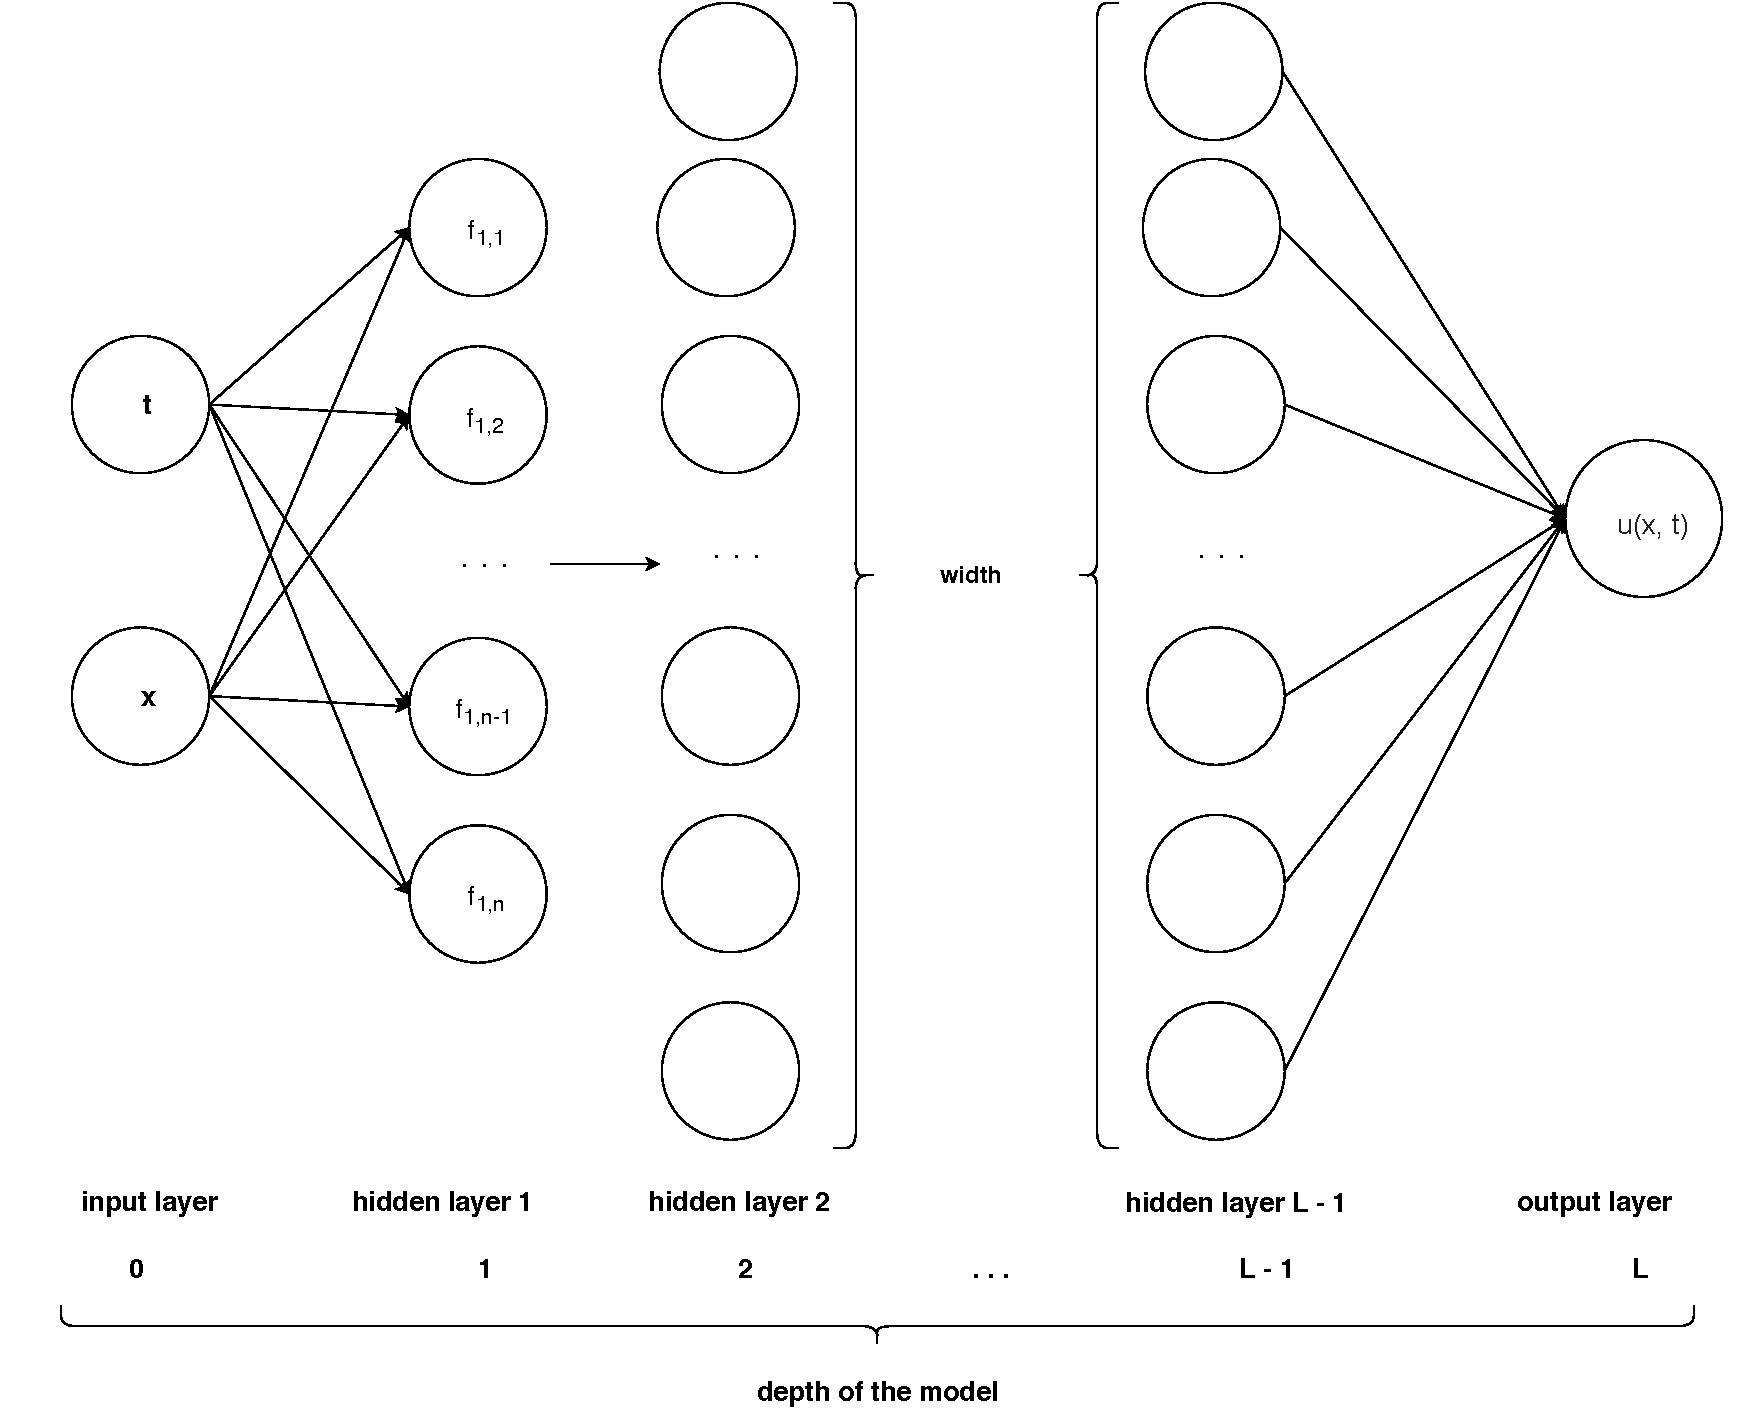
\includegraphics[width = 10cm , height = 7cm]{images/FFNN.pdf}
\\
\caption{Feed forward neural network.}
\end{figure}
\end{frame}

%slide 8
\begin{frame}

As one can see on the Figure 1., we use the first layer as input data driven
form the equation (1). As an activation function, we use $\sigma = tanh(z)$. We
use $tahn(z)$ as its derivative has a good behavior in the region $[-1, 1]$
\cite{nndesign}. In total, the neural network has 10 layers. 6 of them have a
width of 20 "neurons". Below, we will show the dependence of the resulting value
$\lambda$ on the neural network configuration. Especially, the affection of the
number of hidden layers in the network. Below, for the Burgers' equation, the dependence of the result on the neural network configuration was considered.
    
\end{frame}

% Common part (end)
% ------------------------------------------------------------------------------


% ------------------------------------------------------------------------------
% Heat equation part

\section{Example 1. Heat equation}

\begin{frame}{Heat equation}
    We consider the linear heat equation with homogeneous Dirichlet boundary
    conditions
\begin{align*}
    &u_t - \lambda u_xx - g(x, t) = 0, \quad x\in[-1; 1], \quad t\in[0, 1] \\
    &u(x, 0) = 0 \\
    &u(0, x) = u(1, x) = 0
\end{align*}
with source term $g(x, t) = (4\pi^2 -1) \, \sin(2\pi x) \, \exp(-t)$.

True value of $\lambda$ is 1.
\end{frame}

\begin{frame}{Observations}
The exact solution $u = \sin(2\pi x) \, \exp(-t)$ is given on the uniform grid
with 201 points in $x$ and 101 points in $t$. 
We sample 3200 observations uniformly.

\centering
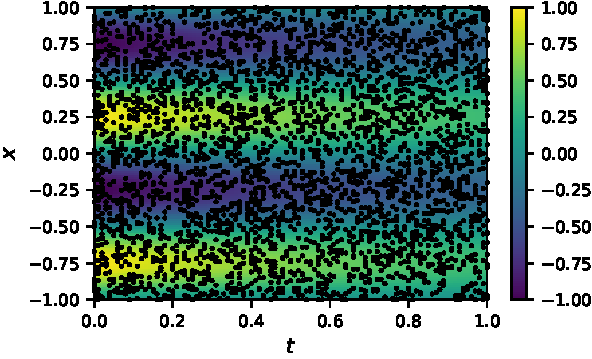
\includegraphics{images/heateq-observations}
\end{frame}

\begin{frame}{Preliminary results with $\gamma=2$}
Training the network with $\gamma=2$ gives prediction $\widehat{\lambda} =
1.00175$ with error $\approx 0.18 \,\%$.

\vspace{0.5cm}
\centering
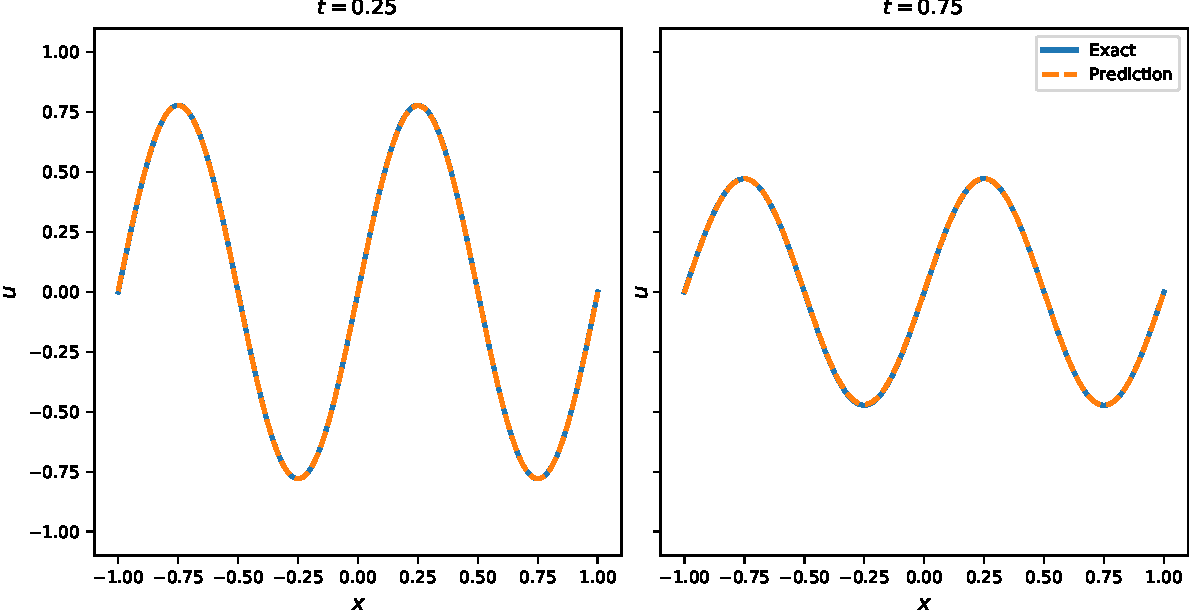
\includegraphics[scale=0.55]{images/heateq-predictions}

\end{frame}

% Heat equation part (end)
% ------------------------------------------------------------------------------


% ------------------------------------------------------------------------------
% Burgers' equation

\section{Example 2. Burgers' equation}

\begin{frame}{Burgers' equation}
In this project we are going to consider the input data of the following form of
the Burgers' equation:
\begin{align*}
&u_t + \lambda_1 u u_x - \lambda_2 u_{xx} = 0, \quad x\in[-1, 1], \quad t\in[0, T]\\
&u(0, x) = -\sin(\pi x) \\
&u(t, -1) = u(t, 1) = 0
\end{align*}

with true values of the sought-for parameters
\[
    \lambda_1 = 1,  \quad \lambda_2 = (0.01 / \pi) \approx 0.318.
\]
{\color{red} The next paragraph is super heavy.
First of all, $N$ is the number observations, do not reuse
the letter for a different purpose.
Call the dimension of $\theta$, for example, $M$.
Second, explain better: in the input layer there are two
neurons, but they do not affect $\theta$; not ``units'' but ``neurons''.
May be, even make a separate slide on how your network
is structured, and how the number of observations is affected.
}

For this problem 3700 observations were used. The optimal number of them is: $2*N^2$, where $N$ is the number of model parameters. As we have 2 input layers, 40 - units in the hidden layers and 1 output layer, we get 3700.

%{\color{red}Write how many observations you take and how}

\end{frame}

\begin{frame}{Observations}
\small
{\color{red}What is $\nu$ in the below formula?}
The exact solution $u(t, x) = \frac{\pi \nu}{\pi \nu exp{\{\pi^2 \nu t\}} - (exp{\{\pi^2 \nu t\}} - 1) cos(\pi x)}$ is given on the uniform grid with 201 points in $x$ and 101 points in $t$. 
\begin{figure}
    \centering
    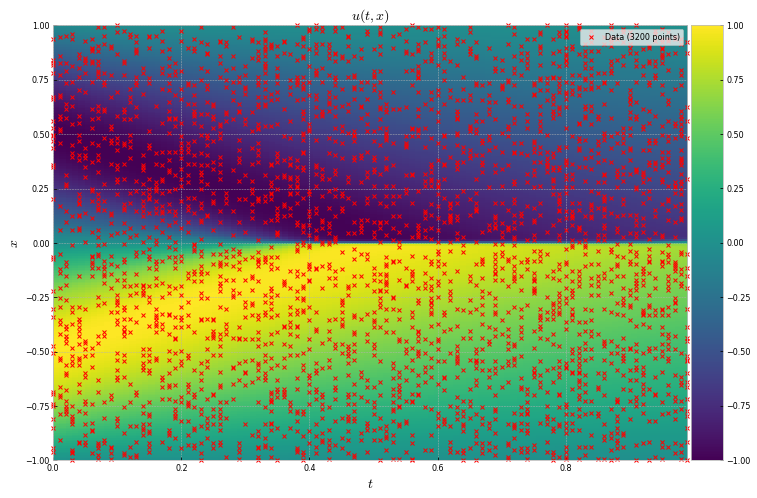
\includegraphics[width=10cm, height=6cm]{images/burgers-exact.png}
    \caption{The exact solution of Burgers' equation and 3700 observations.}
    \label{fig:my_label}
\end{figure}

\centering
%\includegraphics{images/burgers-observations}
\end{frame}

\begin{frame}{Results with $\gamma=0.02553$}
Below, we present a comparison between the exact and the predicted solutions at different time instants t = 0.25, 0.50, 0.75. Training the network with $\gamma=0.0255$ gives prediction $\lambda_1 =
0.986564, ~ \lambda_2 = 0.00338$ with error $\approx 0.094 \,\%$.
{\color{red}Swap with the next slide}

\begin{figure}
    \centering
    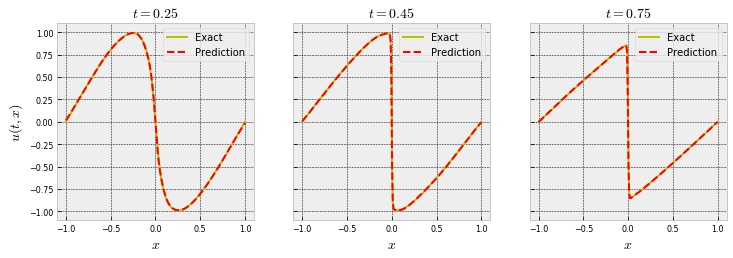
\includegraphics[scale=0.43]{images/burgers-exact-predict.png}
    \caption{The exact and predicted solutions of Burgers' equation in time.}
    \label{fig:burgers-exact-predict}
\end{figure}

\end{frame}

\begin{frame}

Hyperparameter $\gamma$ for the optimization problem was computed via cross-validation technique, using 5 folds. 
\begin{figure}
    \centering
    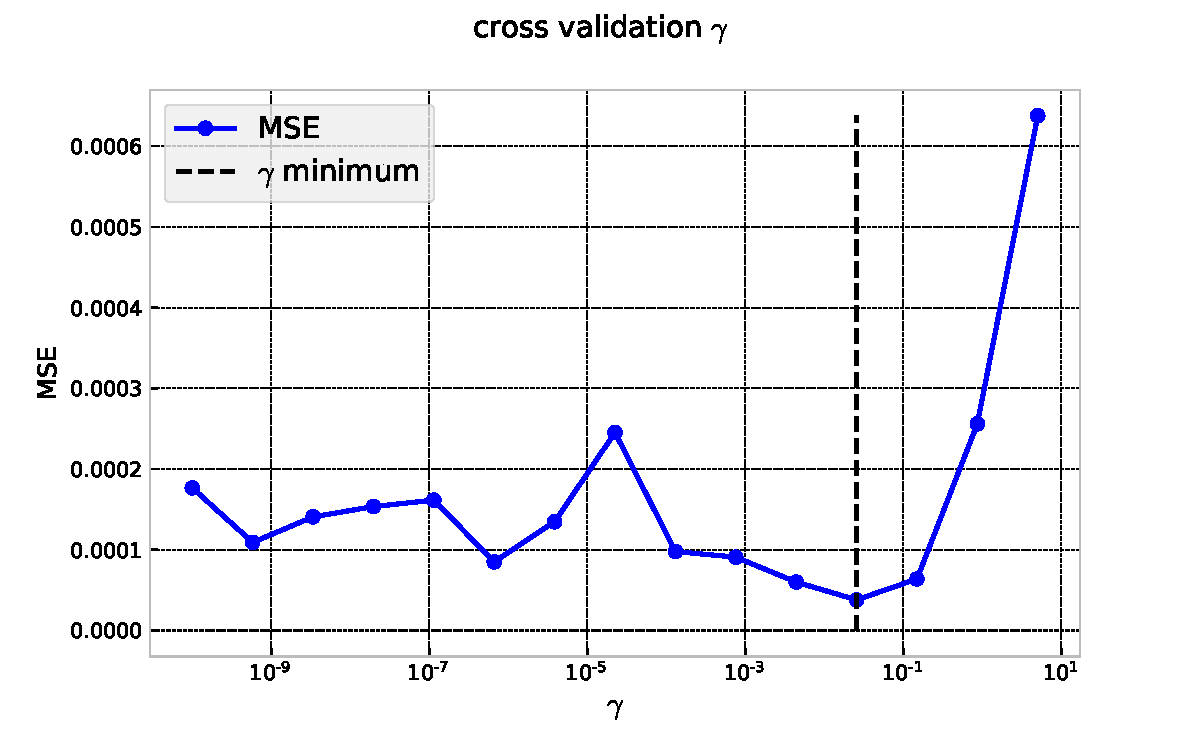
\includegraphics[width=11cm, height=6cm]{images/cross_val_gamma.pdf}
    \caption{Cross-validation result for the hyperparameter $\gamma = 0.0255$.}
    \label{fig:cross_val_gamma}
\end{figure}
    
\end{frame}

\begin{frame}{}

{\color{red}On this and the next slide fix the ratio of the plots and remove
the text about BFGS}
Optimizing loss functions using L-BFGS (a quasi-Newton, full-batch gradient-based optimization algorithm \cite{Liu1989Nocedal}), we have got the following bootstrapped results:
\begin{figure}
\centering
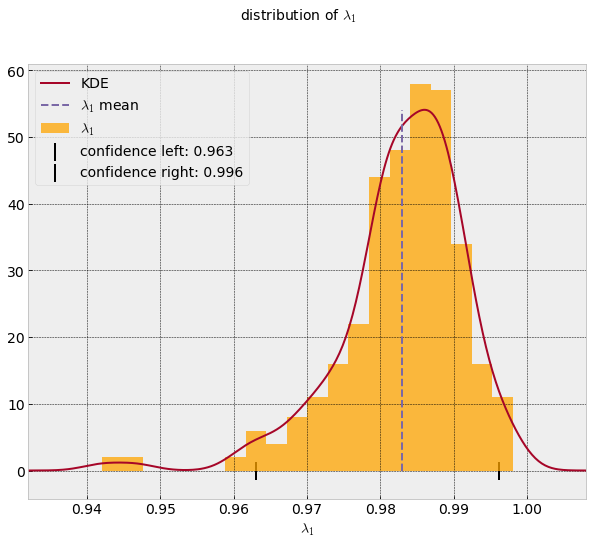
\includegraphics[width = 9cm , height = 6cm]{images/bootstraped_l1.png}
\caption{Bootstrapped parameter $\lambda_1$ for Burgers' equation.}
\end{figure}

\end{frame}

\begin{frame}

\begin{figure}
    \centering
    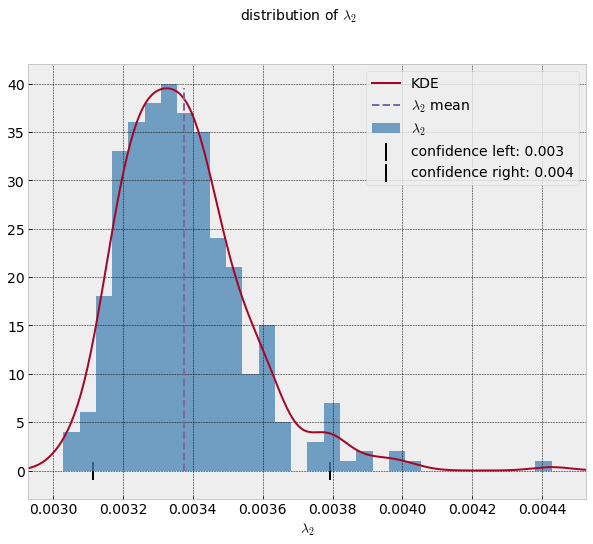
\includegraphics[width = 10cm , height = 7cm]{images/bootstraped_l2.png}
    \caption{Bootstrapped parameter $\lambda_1$ for Burgers' equation.}
    \label{fig:bootstraped_l2}
\end{figure}
    
    
\end{frame}

\begin{frame}{Neural Network configuration $\lambda$ error}

Below one can see the \% error in $\lambda_1$ and $\lambda_2$ for different neural network configurations. In the first column the number of the hidden layers is presented, in the second row the number of the neurons in each hidden layer is presented.

{\color{red} leave only two digits after decimal point.}
\begin{tabular}{lcccccc}
    \toprule
    & \multicolumn{3}{c}{\% error in $\lambda_1$} & \multicolumn{3}{c}{\% error in $\lambda_2$}\\
  \midrule
%  \diagcell{.2em}{1.4cm}{\tiny{Layers}}{\tiny{Neurons}}
\diaghead{Columnmnm}{Layers}{Neurons} & 5 & 10 & 20 & 5 & 10 & 20 \\
\midrule
  1 & 18.917 & 18.769 & 36.789 & 83.962 & 37.824 & 5.327\\
  \hline
  2 & 23.485 & 8.261 & 2.786 & 50.083 & 41.800 & 14.808\\
  \hline
  4 & 7.726 & 1.396 & 2.259 & 1.012 & 3.729 & 0.000065\\
  \hline
  6 & 3.832 & 2.542 & 0.413 & 1.325 & 1.902 & 1.125\\
  \hline
  8 & 9.891 & 1.094 & 2.386 & 52.670 & 4.484 & 2.645\\
  \bottomrule
\end{tabular}
    
\end{frame}

\begin{frame}{Neural Network solution error}

Below one can see the \% error in solution for different neural network configurations. In the first column the number of the hidden layers is presented, in the second row the number of the neurons in each hidden layer is presented.

\centering
    \begin{tabular}{||l|c|c|c||}
        \hline
        & \multicolumn{3}{c}{\% error in solution $u$} | \\
        \hline
        \hline
        & 5 & 10 & 20  \\
        \hline
        1 & 0.190929 & 0.165375 & 0.123150 \\
        \hline
        2 & 0.075636 & 0.036284 & 0.017527 \\
        \hline
        4 & 0.020500 & 0.009551 & 0.008273 \\
        \hline
        6 & 0.014687 & 0.010844 & 0.006640 \\
        \hline
        8 & 0.038927 & 0.007426 & 0.008953 \\
        \hline
    \end{tabular}
\end{frame}

% Burgers' equation (end)
% ------------------------------------------------------------------------------

\begin{frame}
    \frametitle{Conclusions}
    
Therefore, a key property of physics informed neural networks is that they can be effectively trained using small data sets; a setting often encountered in the study of physical systems for which the cost of data acquisition may be prohibitive.

\end{frame}


\bibliography{presentation}
\bibliographystyle{abbrv}

\end{document}
